

\chapter{seL4 Basics}


So far we have provided a general background on real-time scheduling and resource sharing.
Finally we will present the temporal behaviour of our implementation platform, seL4.

seL4 is a microkernel that is particularly suited to safety-critical, real-time systems with one major caveat: the lack of real-time scheduling support. 
Three main features of seL4 support this claim: it has been formally verified for correctness~\citep{Klein_EHACDEEKNSTW_09} and other properties~\citep{Sewell_WGMAK_11}; All memory management, including kernel memory, is all at user-level~\citep{Elkaduwe_Derrin_06}; Finally it is the only \gls{OS} to date with full \gls{WCET} analysis~\citep{Blackham_SCRH_11}.
The scheduler in seL4 has been left intentionally underspecified~\citep{Petters_EH_12} for later work and as a result has a very informal notion of time.
The current implementation is a placeholder, and follows the traditional L4 scheduling model~\citep{Ruocco_06} --- a fixed-priority, round-robin scheduler with 256 priorities.

Systems can currently choose between a restrictive implementation of temporal isolation or a system that presents timing behaviour that is impossible to analyse beyond trivial examples\footnote{Whether analysis is possible in a trivial example beyond one thread is questionable.}.
In this section we will present the current state of relevant seL4 features in order to highlight deficiencies and motivate our changes.
We will outline the scheduler, the API curiosity that is \yield, and how \gls{IPC} interacts with scheduling, followed by an analysis of how the current mechanisms can be used in real-time systems.

\section{Capabilities}
%TODO{define capability}
%TODO{how are they good for mixed criticality}
%TODO{reference EROS, KeyKos}

\section{Kernel memory management}
%TODO{Talk about kernel memory management in seL4, why it is important to keep for mixed criticality systems, and how it complicated designs.}

\section{Scheduler}

The scheduler in seL4 is priority-based round-robin with 256 priorities (0 --- 255), implemented as an array of lists: one list of ready threads for each priority level. 
At a scheduling decision, the kernel chooses the head of the highest-priority, non-empty list, and removes it from the relevant scheduler queue, which is referred to as \emph{benno Scheduling}.
The kernel previously used \emph{lazy scheduling}, leaving the current thread in its run queue, however this was replaced in favour of Benno scheduling to reduce the WCET of the kernel. 
This is different to a previous kernel implementation which left the currently running thread in its run queue, however this increased the kernels \gls{WCET} and was removed.

Scheduling decision complexity is $O$(number of priorities), as the algorithm searches for a non-empty list from the highest priority down, however can easily be optimised to $O(1)$, as a 2-level bit field can track the highest runnable priority\footnote{This feature exists in a branch but is not yet verified}. 

Kernel time is accounted for in ticks, with a static tick length defined at compile time (CONFIG\_TIMER\_TICK\_MS).
Threads have a timeslice field which represents the number of ticks they are eligible to run. 
This value is decremented every time a timer tick is handled, and when the timeslice is exhausted the thread is appended to the relevant scheduler queue, with a replenished timeslice.
The reload value of the timeslice is also defined at compile time (CONFIG\_TIME\_SLICE).

In an unrealistically simple system, where threads run at the same priority and do not communicate, it is possible to analyse temporal behavior on seL4: threads will run for the timeslice value in round-robin order.
However, the allocation of ticks to threads is not actually that simple due to yield behaviour, preemption and \gls{IPC}. 

\subsection{seL4\_Yield}

The presence of the \yield system call complicates timing analysis.
In the traditional L4 interface, yield was the mechanism for timeslice donation. 
In seL4 this is not the case, as \texttt{seL4\_Yield} simply appends the currently running thread to the appropriate scheduling queue and selects the new head as runnable \textit{without altering the timeslice value}.
As a result, if only 1 tick is left in the yielding thread, when the thread is next scheduled it will run for 1 tick, rather than \texttt{CONFIG\_TIME\_SLICE}, and consequently yield simply donates the remainder of the current tick and alters scheduling ordering.

Although the behaviour of yield is confusing and results in interesting scheduling behaviour, it does not actually violate temporal isolation, as threads can conspire to give each other more time, but they cannot take time away from other threads.
This behaviour is considered a specification bug, not a feature. 

In practice, yield is useful for implementing in-memory spin locks, or to ensuring intended scheduling ordering during benchmarks.

\subsection{Priorities}

Like any priority-based kernel without temporal isolation mechanisms, time is only guaranteed to the highest priority threads.
Priorities in seL4 act as informal capabilities: threads cannot create threads at priorities higher than their current priority, but can create threads at the same or lower priorities.
If threads at a higher priority levels never block, lower priority threads in the system will not run.
As a result, a single thread running at the highest priority has access to 100\% of processing time.
However, even this becomes unclear once there is more than one thread at a priority: if two threads are running, they can both access 50\% of processing time.
If one of two threads blocks, the other gets 100\% of processing time and vice versa.
There is no way to enforce a certain processor allocation and how CPU time a thread receives is up to priorities and the behavior of other threads in the system, which is impossible to guarantee.

\subsection{IPC Interaction}

\gls{IPC} complicates the timing behaviour of the kernel further.
When a \gls{IPC} is sent to a higher priority thread, that thread is switched to immediately.
For a lower priority thread, the scheduler is invoked and the thread will only be scheduled if no other high priority threads are runnable.

In the case where the \gls{IPC} is to a thread at the same priority, the round-robin scheduler queue at that priority is bypassed and the thread is switched to immediately.
Note that other threads in the scheduling queue are not starved, as when one of the rendezvous partners exhausts its timeslice the scheduler will choose the next round-robin thread.
However, \textit{when} this happens is not deterministic.

We can demonstrate the non-deterministic scheduling ordering as a result of IPC with an example.
Consider the case where threads $A$ and $B$, both at the same priority, and are exchanging IPC messages constantly.
Another thread $C$ is running at the same priority, and all threads have full timeslice fields.
$C$ will be scheduled when one threads timeslice is exhausted, i.e when either $A$ or $B$ has been preempted \texttt{CONFIG\_TIME\_SLICE} times.
As a result $C$ could be scheduled after at minimum \texttt{CONFIG\_TIME\_SLICE} ticks (if one of the \gls{IPC} partners is preempted for every tick, or at maximum after \texttt{CONFIG\_TIME\_SLICE * 2 - 1} ticks (if both partners are preempted for ticks).
This example is illustrated in \cref{fig:non-determinism}.

\begin{figure}
    \centering
    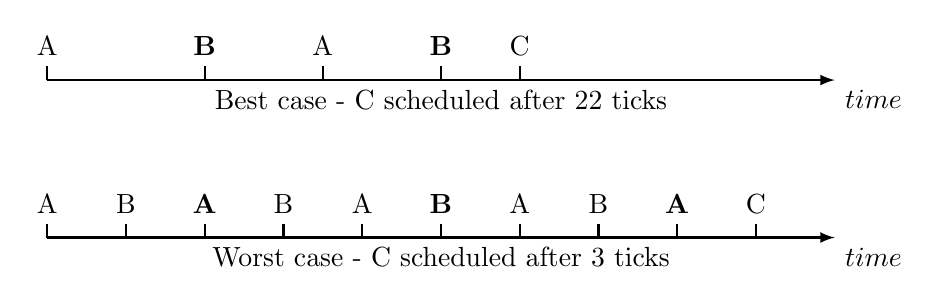
\begin{tikzpicture}[x=1cm]

        \draw[->,thick,>=latex] (0,0) -- (10,0) node[below right] {$time$};
        \draw[thick] (0,0) -- ++(0,5pt) node[above] {A};
        \draw[thick] (1,0) -- ++(0,5pt) node[above] {B};
        \draw[thick] (2,0) -- ++(0,5pt) node[above] {\textbf{A}};
        \draw[thick] (3,0) -- ++(0,5pt) node[above] {B};
        \draw[thick] (4,0) -- ++(0,5pt) node[above] {A};
        \draw[thick] (5,0) -- ++(0,5pt) node[above] {\textbf{B}};
        \draw[thick] (6,0) -- ++(0,5pt) node[above] {A};
        \draw[thick] (7,0) -- ++(0,5pt) node[above] {B};
        \draw[thick] (8,0) -- ++(0,5pt) node[above] {\textbf{A}};
        \draw[thick] (9,0) -- ++(0,5pt) node[above] {C};
   
        \node[below,align=left,anchor=north,inner xsep=0pt] at (5,0) 
            {Worst case - C scheduled after 3 ticks};  
    
        \draw[->,thick,>=latex] (0,2) -- (10,2) node[below right] {$time$};
        \draw[thick] (0,2) -- ++(0,5pt) node[above] {A};
        \draw[thick] (2,2) -- ++(0,5pt) node[above] {\textbf{B}};
        \draw[thick] (3.5,2) -- ++(0,5pt) node[above] {A};
        \draw[thick] (5,2) -- ++(0,5pt) node[above] {\textbf{B}};
        \draw[thick] (6,2) -- ++(0,5pt) node[above] {C};

        \node[below,align=left,anchor=north,inner xsep=0pt] at (5,2) 
            {Best case - C scheduled after 22 ticks};  
    \end{tikzpicture}
    \caption{Non-deterministic scheduling in the case of IPC and variable execution times. A and B are IPC partners, C is a third thread. A, B and C run at the same priority. \texttt{CONFIG\_TIME\_SLICE} is 2. Bold indicates the thread that is preempted by the timer tick. In the best case, B takes both timer ticks and C is scheduled after 2 ticks. In the worst case, A takes 2 ticks and B takes 1, such that C is scheduled after 3 ticks.}
    \label{fig:non-determinism}
\end{figure}

\subsection{Domain scheduler}

A recent addition to the seL4 kernel adds the ability to guarantee complete temporal isolation and deterministic scheduling between sets of threads, using the concept of scheduling \emph{domains}.
Threads are assigned to domains, each of which has a separate array of lists of threads over the priority range.
Each domain runs for a fixed amount of ticks, and domains are scheduled sequentially and deterministically.
Cross-domain \gls{IPC} and yielding is not permitted, and even if there are no runnable threads while a domain is scheduled, the idle thread will run until a domain switch occurs.

The domain scheduler can be leveraged to achieve temporal isolation however since domains cannot be preempted, it would only be useful for cyclic, non-preemptive scheduling with scheduling order and parameters computed offline and no resource sharing.
In such a scenario each real-time task could be mapped to its own domain, and each task would run for its specified time before the domain scheduler switched to the next thread.
Any unused time in a domain would be wasted, and spent in the idle thread.

However, in such a scheduler is only suitable for closed systems where resource sharing is not required, and results in low system utilisation.
Dynamic real-time applications with shared resources and high system utilisation are not compatible with the domain scheduler, as they require preemption.

\section{Summary}

We have covered seL4 mechanisms that affect timing behaviour in the kernel: the scheduler, priorities, yield and IPC. 
In this section we will look at how real-time scheduling could be implemented with those mechanisms.

There are several options for implementing a real-time scheduler in the current version of seL4: leveraging the domain scheduler, using the priority scheduler or implementing a scheduling component to run at user-level. 
As the previous section established, the domain scheduler offers low utilisation for strictly closed systems without resource sharing, so is clearly insufficient.

The priority scheduler could be leveraged to implement a rate-monotonic scheduler.
However, this requires complete trust in every thread in the system, as there is no mechanism for temporal isolation: if one thread executes for too long, other threads will miss their deadlines.
Essentially the only thread with a guaranteed CPU allocation is the highest priority thread, which under rate-monotonic priority assignment is not the most critical thread in the system, but the thread with the highest rate.
Additionally, periodic threads driven by timer interrupts rather than events would need to share a user-level timer.

\begin{table}
	\centering
	\begin{tabular}{| l | p{2cm} | p{2cm} | p{2cm} | p{2cm} |} \hline
		                  & Temporal isolation & Utilisation & Low kernel overheads & Dynamic\\\hline
Domain scheduler          & \yes               & \no         & \yes        & \no    \\\hline
Priority scheduler        & \no                & \yes        & \yes        & \yes   \\\hline
Trusted timer component   & \yes               & \yes        & \no         & \yes   \\\hline
	\end{tabular}
	 \caption{Comparison of existing seL4 scheduling options -- nothing ticks all of the boxes.}
	 \label{tab:nothing-ticks-all-boxes}
\end{table}


To build a dynamic system with temporal isolation and high CPU utilisation, one could implement a trusted timer component at user-level.
This component would be the highest priority thread in the system, and could pause threads to prevent them from overrunning their assigned rate.
However, since the timer component would need to maintain accounting information and track the currently running thread, it would need to be invoked for every single scheduling operation.
This is prohibitively expensive, as it results in doubled context switching time and increased number of system calls for thread management.

\Cref{tab:nothing-ticks-all-boxes} shows a comparison of all of the available scheduling options in the current version of seL4 -- no option provides all of the qualities we require.
Clearly, the kernel needs something more. 
In the next section we will outline our design for a more principled approach to time for seL4 -- using the principles of resource kernels and with the aim of support diverse task sets, including those for mixed-criticality systems.

